\documentclass{article}
\usepackage{amsmath}
\usepackage{caption}
\usepackage{placeins}
\usepackage{graphicx}
\usepackage{subcaption}
\usepackage{tikz}
%\usepackage[active,tightpage]{preview}
\usepackage{natbib}
\bibpunct{(}{)}{,}{a}{}{;} 
\usepackage{url}
\usepackage{nth}
\usepackage{authblk}
% for the d in integrals
\newcommand{\dd}{\; \mathrm{d}}
\newcommand{\tc}{\quad\quad\text{,}}
\newcommand{\tp}{\quad\quad\text{.}}

\begin{document}

\title{Distributional aspects of time to death in human populations}

\author[1]{Tim Riffe}
\author[2,3]{Adam Lenart}
\author[2,3]{Vladimir Canudas Romo}
\affil[1]{Department of Demography, University of California, Berkeley}
\affil[2]{University of Southern Denmark}
\affil[3]{Max Planck Odense Center}


\maketitle

\section{Background}

Typically demographers are satisfied to summarize the remaining lifetime for age
groups using a mean, $e(a)$, which is however not an omnibus descriptor of time
to death. There are other useful measures of longevity, such as
the modal or median ages at death, and demographers also have a battery of
indicators for lifespan variability or entropy. One aspect in common of all
these indicators except for remaining life expectancy is that they refer to the
age distribution of mortality in a snapshot of a stationary population or else
the age at death distribution of a newborn cohort under constant mortality
conditions. These measures are not typically made conditional on survival to
later ages, i.e., demographers too seldom consider the properties of the
distribution of remaining lifetimes as a function of age itself. All of
the above measures can be reworked as functions of conditional remaining
lifetime (e.g., the modal remaining lifespan) to become functions of age.
In this paper, we aim to provide some elementary definitions and
apply these to human populations. As an example of utility of this perspective we offer a
selection of simple heuristics for late life decisions based on these
distributional measures.

\section{Definitions}

Remaining life expectancy conditional on survial to age $a$ is defined as
\begin{equation}
e(a) = \frac{\int_{y=0}^\infty l(a+y) \dd y}{l(a)} \tp
\end{equation}

Say lifespans for a given birth cohort are measured with the random variable,
$X$, with distribution $d(X)$, which is identical to the $d_x$
column of the lifetable if a radix of 1 is used. In other words, the
distribution of lifespans for newborns is identical to the distribution of
age at death in the stationary population. We are interested in the
conditional density function, $f(X-a ~|~ X \ge a)$, which we denote using
$f(y|a)$, and which is defined as:
\begin{equation}
\label{eq:fya}
f(y|a) = \mu(a+y) \frac{l(a+y)}{l(a)} \tc
\end{equation}
i.e., the probability of surviving to and dying at age $a+y$ given survival to
age $a$. \eqref{eq:fya} can also be used to calculate remaining life expectancy:
\begin{equation}
e(a) = \int _{y=0}^\infty y f(y|a) \dd y \tp
\end{equation}

Demographers make less frequent
reference to $f(y|a)$, which is however useful for decomposing
demographic counts into remaining lifetime classes. The empirical distribution
of $f(y|a)$ is a worthy topic of study, as it bears heavily on many late-life
decisions, such as bequesting or moving into a care residence, and possibly also
on the ethical pondering of public policies, such as mandatory retirement ages
or pensions. The conditional distribution of remaining lifetimes can be
described empirically using quantiles, or other central measures such as the
median or the mode, or perhaps more parsimoniously using standardized moments.

The $n^{th}$ moment about the conditional mean of $f(y|a)$,
$\eta_n(y|a)$ is defined as:
\begin{align}
\eta _n(y|a) =& \frac{1}{l(a)} \int_{y=0}^\infty (y-e(a))^n \mu (a+y) l(a+y) \dd
y 
\intertext{or just}
\eta _n(y|a) =&  \int_{y=0}^\infty (y-e(a))^n f(y|a) \dd y \tc
\end{align}
where $\eta_2(y|a)$ gives the variance of remaining lifespan about $e(a)$,
$\sigma^2(y|a)$. Survival-conditioned variance is useful information, but it can be deceptive to display graphically, since lifespan variation
is not usually symmetric around $e(a)$. The conditional skewness function is not
a perfect measure of symmetry in $f(y|a)$, but it captures most such varation
and can be roughly interpreted in this way. is calculated as:
\begin{equation}
\frac{\eta_3(y|a)}{\eta_2(y|a)^{\frac{3}{2}}} \tc
\end{equation}
the third standardized moment. The fourth standardized moment, the conditional
kurtosis of $f(y|a)$, is defined as (find appropriate notation for skewness and
kurtosis)
\begin{equation}
\frac{\eta_4(y|a)}{\eta_2(y|a)^2} \tp
\end{equation}
The coefficient of variation of remaining lifespan, $CV(y|a)$ is then simply
\begin{equation}
CV(y|a) = \frac{\sqrt{\eta_2(y|a)}}{e(a)} \tp
\end{equation}
$CV(y|a)$ is dimensionless and comparable over age, and its reciprocal
can be thought of as a signal to noise ratio of one's likely remaining lifespan,
assuming a constant mortality pattern in ages higher than $a$.

L-moments\citep{hosking1990moments} may also be calculated for the the lifetable
conditional distribution of remaining lifetimes. These measures yield qualitatively similar reslts, but
are more robust to noise and outliers, and they are also appropriate for ordered
vaiables such as age-classified mortality functions. Tyically L-moment
calculation proceeds from individual-level data, which is never drawn from
a stationary population. Here we present the general L-moment formulas for
grouped data, which can be applied to the standard lifetable if specified with a
large radix, such as the HMD standard of $100,000$, or possibly more
appropriately to a radix the size of the theoretical stationay birth cohort
that would yield the same popuation size as that observed in the year to which
the lifetable refers (Adam, am I way off?).

definition goes here:

\section{Observed patterns}
The above definitions are exact and amenable to calculation from
the standard lifetable.To begin, let us
compare some percentiles of the distribution of $f(y|a)$, translated to
$f(a+y|a)$. Figure~\ref{fig:IQR1} provides shows the median and interquartile
range of conditional age attained implied by period rates for Swedish females in
1900 and 2000. In a general sense, we can conclude from this Figure that the
lower quantiles of conditional age attained change much more over age than do
upper quantiles. We also see that lower mortality regimes year (2000) have more
compact interquartile ranges than to do high mortality regimes (1900), meaning
that one can wager an age at death with greater certainty. Further, in
contemporary low mortality regimes, with low early life mortality, the
conditional IQR holds nearly constant (in fact it always rises, albeit
imperceptibly) until after typical midlife ages.
% Figure produced in R/GeneralPatterns.R
\begin{figure}[h!]
\centering
	\caption{Sweden females, 1900 and 2000. \nth{25}, \nth{50}, and \nth{75}
	percentiles of conditional survival, given period mortality (HMD)}
	\label{fig:IQR1}
	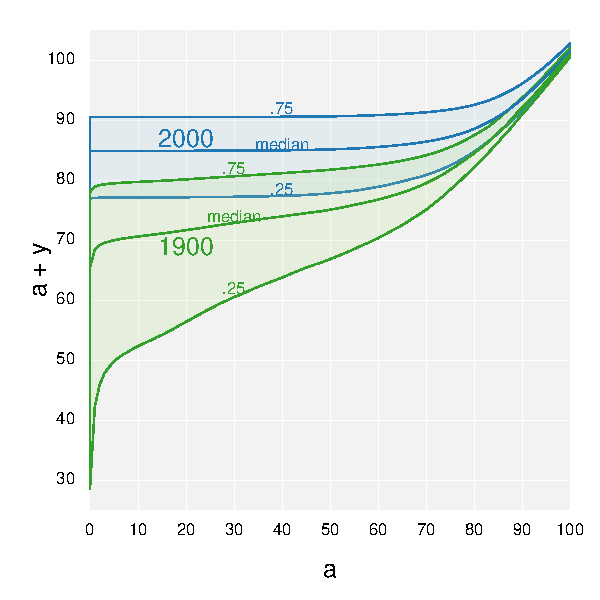
\includegraphics[scale=.7]{Figures/SwedenFemalesIQR1900_2000.pdf}	
\end{figure}

Likewise, what is the age where inequality in remaining lifespan is at its
minimum, and how stable is this age over time and between populations?

\section{Heuristics}
Ceteris paribus (i.e., in a homogenous population and where investment
specifics do not play in), negative skewness suggests that we buy an (actuarily
fair) annuity and positive skewness implies that the odds of us surviving to get 
the money back are less than unity?

What would the ethicist say about the just span of retirement? The variance of
time to death is not monotonic, but instead decreases until some late age and
then increases again. Could a just age of mandatory retirement be the age where
the variance in remaining lifespan is at a minimum? To equalize the duration of
retirement between individuals is at first glance a step toward equality, but
there is no anecessary or best way to determine this duration, and there is also
no necessary way to adjust this duration as a function of lifespan itself. In
other words, if the desired duration of retirement is 20 years, perhaps the
meaning of 20 years is greater for an individual with a shorter lifespan and
lesser for a longer total lifespan.

Can the age of minimum variance be used as another sort of demographic threshold
for ageing or dependency?

\bibliographystyle{plainnat}
  \bibliography{references}   % Use the BibTeX file ``References.bib''.

\end{document}
